\begin{figure}[H]\centering
    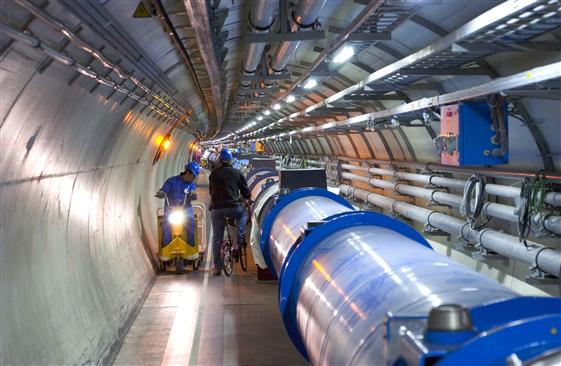
\includegraphics[width=0.6\textwidth]{figure/lhc_tunnel.jpg}
    \caption{LHC tunnel and beam pipe.}
    \label{fig:lhc_tunnel}
\end{figure}
The LHC lies in the already existing 27 km tunnel (Fig.~\ref{fig:lhc_tunnel}) which previously hosted the Large Electron Positron collider (LEP) in the Geneva region and it is as deep as 175 m  beneath the France-Switzerland boarder.
The LHC yields head-on collisions of 7 \TeV for proton-proton beams and the collision energy reach to 13 \TeV with a designated luminosity of $2 \ten{34}$\percms in the LHC RunII period (2015 - 2018).
The prime motivaition of the LHC is to test the predictions of different theories of partilce physics, and have the ability to explore rare evetns such as the Higgs boson production and physics beyond the SM. 

\subsection{Proton injection and operational cycle}
The proton beams goes through series of stages of acceleration (Fig.~\ref{fig:lhc_layout}) to achieve the desired collision energy.
Protons are first produced by linear particle accelerator (LINAC2).
The LINAC2 provides bottles of negative hydrogen ions as the source of the protons, and the electrons are stripped from the hydrogen ions by the electric field leaving only the nucleus containing one proton.
The protons are then boosted up to 50 \MeV, feeding the Proton Synchrotron Booster (PSB) which is the first accelerator in the acceleration chain.
The protons are further speeded up to 1.4 \GeV by four superimposed rings with a radius of 25 m inside the PSB.
The Proton Synchrotron (PS) with 277 conventional (room-temperature) electromagnets can operates the acceleration up to 25 \GeV and provide the bunches with 25 ns to the Super Proton Synchrotron (SPS).
The SPS is the second largest machine in CERN’s accelerator complex, and have the ablility to boost the protons from the PS up to 450 \GeV before they are injected into the main accelerator with the designated energy of 6.5 \GeV
\begin{figure}\centering
    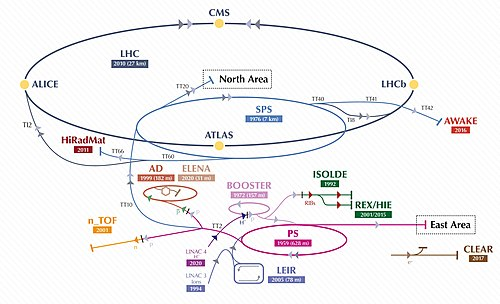
\includegraphics[width=0.8\textwidth]{figure/lhc_layout.jpeg}
    \caption{Schematic layout of the LHC at CERN.}
    \label{fig:lhc_layout}
\end{figure}

\subsection{Machine design}
The LHC contains two adjacent parallel hadron accelerator ring each containing a beam traveling in opposite directions and surrounded by a common cold mass and cryostat, as shown in Fig~\ref{fig:lhc_xsec}.
To avoid the accelerated protons colliding with the air molecules, the pressure in these pipes is \ten{-10} to \ten{-11} mbar, a vacuum almost as rarefied as that found on the surface of the Moon.
Those two rings are designed as twin-aperture magnets containing two contra-rotating beams because of the space limitation in the tunnel.
The beams intersect at four points around the ring, which is where the particle collisions take place.

The LHC is mainly comprised of superconducting magnets and radiofrequency (RF) cavities.
There is about 10 000 superconducting magnets are installed having a mass of over 27 tonnes and all are electromagnets.
A total 1232 main dipole magnets, each 15 meters long, are used to keep the high-energy proton beam on their circular path with a powerful magnetic filed of 8.3 T.
Each dipole magnet is driven by superconducting coils composed of NbTi/Cu rutherford cables.
Approximately 96 tonnes of superfluid helium is needed to keep the magnets at their operating temperature of 1.9 K.
A total 392 quadrupole magnets are allocated symmetrically around the beam pipe to steer the beam in the transverse plane.
To maximize the chances of particle collisions, strongerr quadrupole magnets are used close to the intersection points.
Magnets of higher multipole orders are used to correct smaller imperfections in the field geometry. 
\begin{figure}\centering
    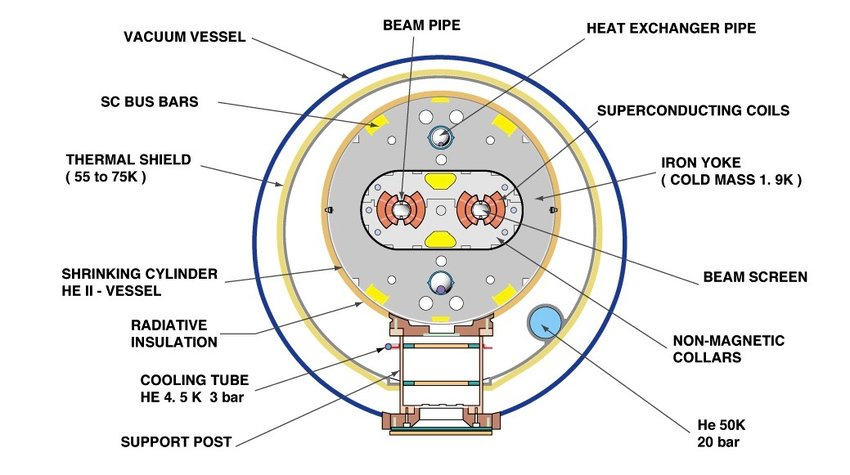
\includegraphics[width=0.8\textwidth]{figure/lhc_xsect.jpg}
    \caption[Cross section of the cryostat system.]
    {Cross section of the cryostat system, where the dipole magnets are surrounded by the superfluid helium.}
    \label{fig:lhc_xsec}
\end{figure}

There are 8 RF cavities per beam pipe on the LHC with a purpose of accelerating the charged particles.
The 16 RF cavities on the LHC are housed in four cylindrical refrigerators called cryomodules which keep the RF cavities working in a superconducting state, without losing energy to electrical resistance.
A RF cavity is a metallic chamber structured like beads on a string, where the string is the beam pipe and the beads are the cavities, shown in Fig~\ref{fig:rf_cavities}.
Each RF cavity is operated with an RF power generator supplying an electromagnetic filed generated from high-power klystrons (tubes containing electron beams).
In order to build up the electromagnetic waves inside the cavity, the RF cavity is molded to a specific shape and size.
The high-power electron beam is extracted through a rectangular pipe of conducting metal called a waveguide, which leads to the RF cavity.
Charged particles passing through the cavity feel the overall force with same direction where the accelerating electromagnetic field oscillates.
It is important to time the arrival of particles since the electromagnetic field is made to oscillate at 400 MHz.
The ideally time proton, with the exact desired energy, will have zero accelerating voltage.
In contrast, protons with slightly different energy from the designated collision energy will be accelerated or decelerated in order to reach to the desired energy and form the proton packs called bunches.
Their accelerating electromagnetic fields can achieve a maximum voltage of 2 MV per cavity (total 16 MV per beam) in the longitudinal direction.
During the energy-boosting process, each injection beam is at 450 \GeV and can be boosted up to top energy in around 15 minutes.
The protons in the bunches have an overall acceleration on each passage through the cavities, and the bunches having passed the cavities around 1 million times at 6.5 \GeV.
\begin{figure}\centering
    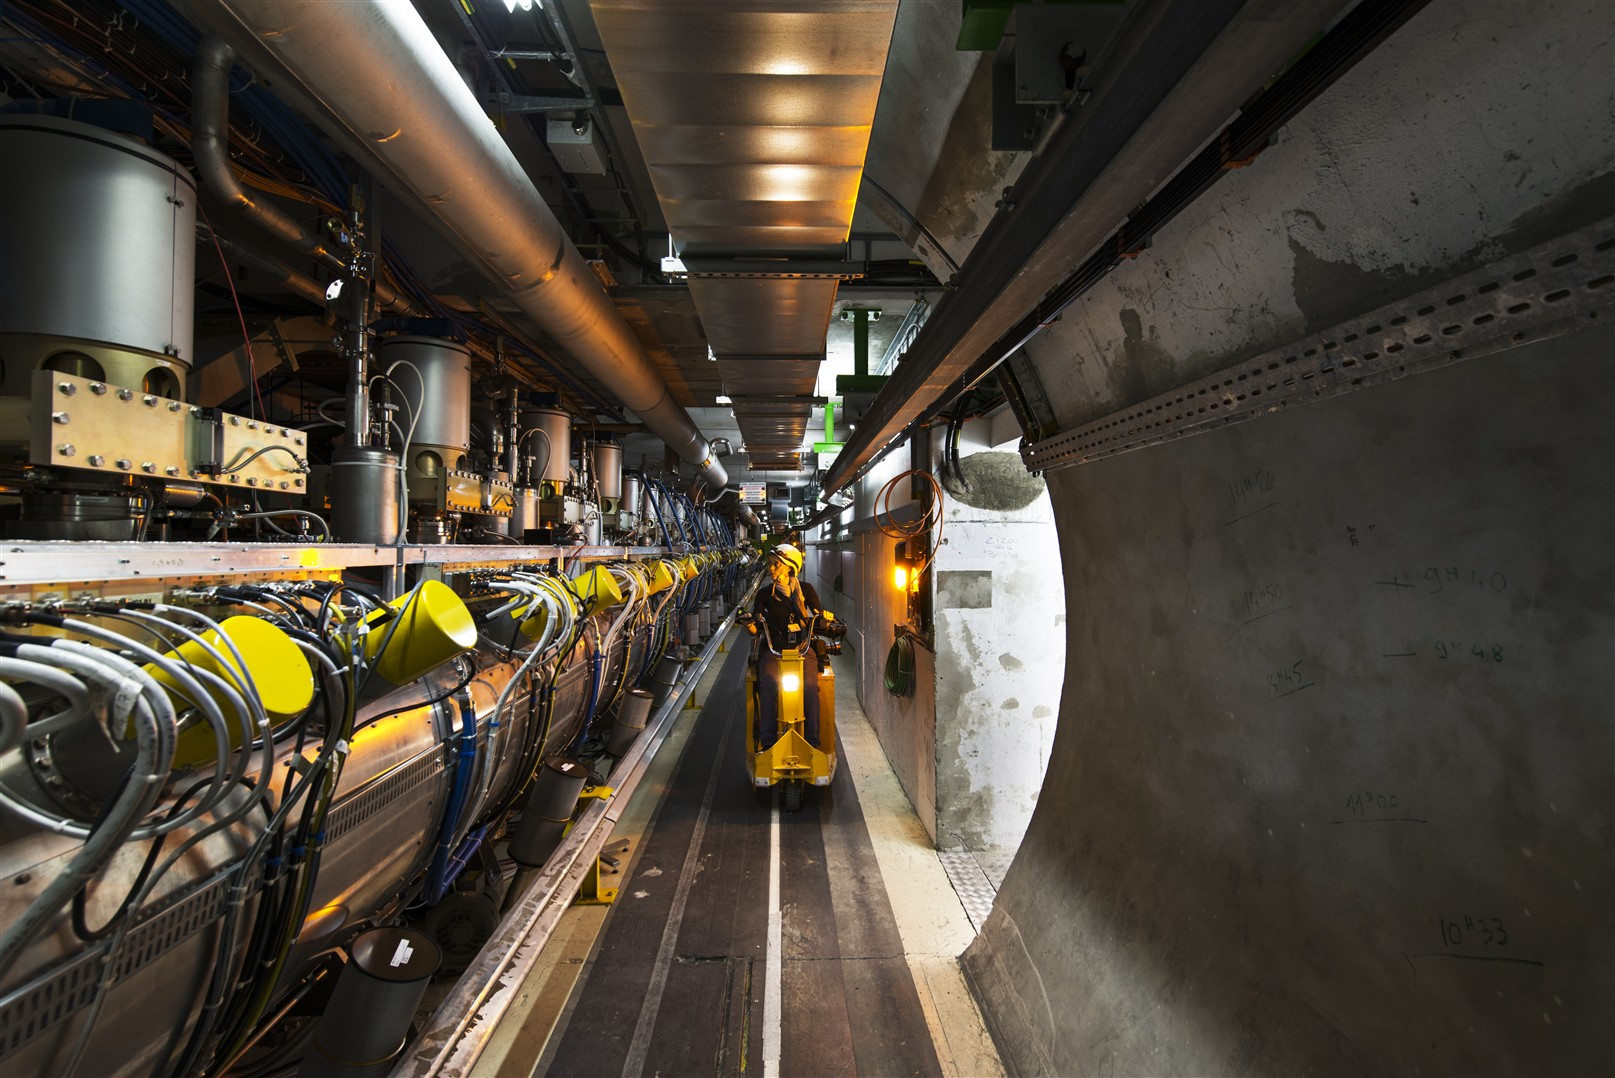
\includegraphics[width=0.8\textwidth]{figure/rf_cavities.jpg}
    \caption{One of the module containing the accelerating cavities for the LHC.}
    \label{fig:rf_cavities}
\end{figure}

The main accelerator is composed of eight arcs and eight straight sections (Fig.~\ref{fig:lhc_arc}).
Either an experimental or utility insertion is located in each straight section.
The two high luminosity experiment, A Toroidal LHC Apparatus (ATLAS) and CMS, are located at Point 1 and Point 5, respectively.
The other experiments, LHC-beauty (LHCb) and  A Large Ion Collider Experiment (ALICE), are located at Point 2 and Point 8, separately.
The utilities containing collimation systems to reduce quenching of superconducting magnets and damage of accelerator components are based on Point 3 and Point 7.
The RV cavity systems for particle acceleration and beam dumping system extracting beams from each ring of the collider can be found at Point 4 and Point 6, respectively.
\begin{figure}\centering
    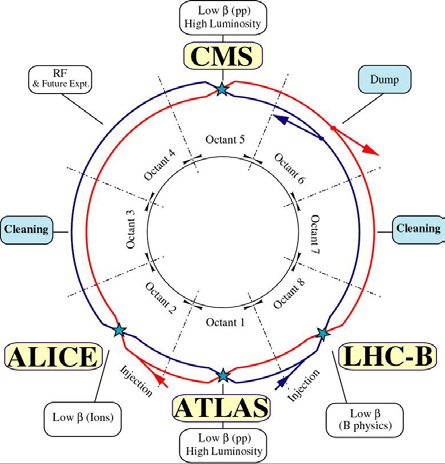
\includegraphics[width=0.5\textwidth]{figure/lhc_arc.png}
    \caption{Schematic layout of the main accelerator for the LHC at CERN.}
    \label{fig:lhc_arc}
\end{figure}

\subsection{Luminosity and pileup}
Luminosity gives a measure of how many collisions are happening in a particle accelerator.
It is an important indicator to reflect the number of collisions that occur in a given amount of time. 
The higher the luminosity, the more data the experiments can gather to allow them to observe rare processes.
The number of events produced per second from a process can be written as
\begin{linenomath}\begin{equation}\label{eq:lumi_nevt}
    N_X = L_0 \sigma_{\pp\rightarrow X}
\end{equation}\end{linenomath}
where $L_0$ is the instantaneous luminosity, $\sigma_{\pp\rightarrow X}$ is the cross section of the $X$ production, and $N_X$ is the number of events.
With the assumption that the proton beam density function follows a normal distribution and the two colliding beams are with the same beam parameters, the instantaneous luminosity can be defined as
\begin{linenomath}\begin{equation}\label{eq:lumi_l0}
    L_0 = \frac{N^2_b n_b f_{\mathrm{rev.}} \gamma_r}{4\pi\hat{\epsilon}\beta^*}F
\end{equation}\end{linenomath}
where $N_b$ is the number of particles per bunch; $n_b$ is the number of bunches per beam; $f_{\mathrm{rev.}}$ is the revolution frequency; $\gamma_r$ is the relativistic gamma factor; $\hat{\epsilon}$ is the normalized transverse beam emittance; $\beta^*$ is collision point of the amplitude $\beta$ function; and $F$ is the geometric luminosity reduction factor. $F$ can be further expressed as
\begin{linenomath}\begin{equation}\label{eq:lumi_F}
    F = \biggl( 1 + \Bigl(\frac{\theta_c \sigma_z}{2\sigma^*}\Bigr)^2 \biggr)^{-\frac{1}{2}}
\end{equation}\end{linenomath}
where $\theta_c$ is the full crossing angle at the interaction point, $\sigma_z$ is the RMS bunch length, and $\sigma^*$ is the transverse RMS beam size at the interaction point.

The LHC cranks up the performance to achieve high instantaneous luminosity at the cost of pileup (PU).
The PU is defined as the average number of particle interactions per bunch-crossing, and can be expressed as
\begin{linenomath}\begin{equation}\label{eq:lumi_pu}
    \bigl< \mu \bigr> = \frac{\mathcal{L}_{\mathrm{inst.}}\sigma^{\mathrm{inel.}}_{\pp}}{n_b f_{\mathrm{rev.}}}
\end{equation}\end{linenomath}
where $\sigma^{\mathrm{inel.}}_{\pp}$ is the inelastic proton-proton cross section with a value of 69.2 mb at \newTeV and $\bigl< \mu \bigr>$ is the PU.
The value of the PU reflects the number of particles produced at the same time, and high PU presents a challenge for physics analyses to successfully identify collisions of interest resulting from signal processes.

The LHC has delivered more than 160 \fbinv overall of proton-proton collisions in Run 2, and the CMS collected more than $92\%$ of the Run 2 data successfully yielding a total dataset of 150 \fbinv.
Figure~\ref{fig:lhc_lumi} shows the integrated luminosities during the LHC Run I and Run II.
The integrated luminosity for physics analysis from 2016 to 2018 is 137 \fbinv and the instantaneous luminosities are 1.4 \percms in 2016 and 2.1 \percms in 2017 and 2018.
The measured PU distribution in the CMS experiment during the LHC Run 1 and Run 2 is shown in Figure~\ref{fig:lhc_pu}.
The machine reached a peak average pileup of around 60 in 2018.
\begin{figure}\centering
    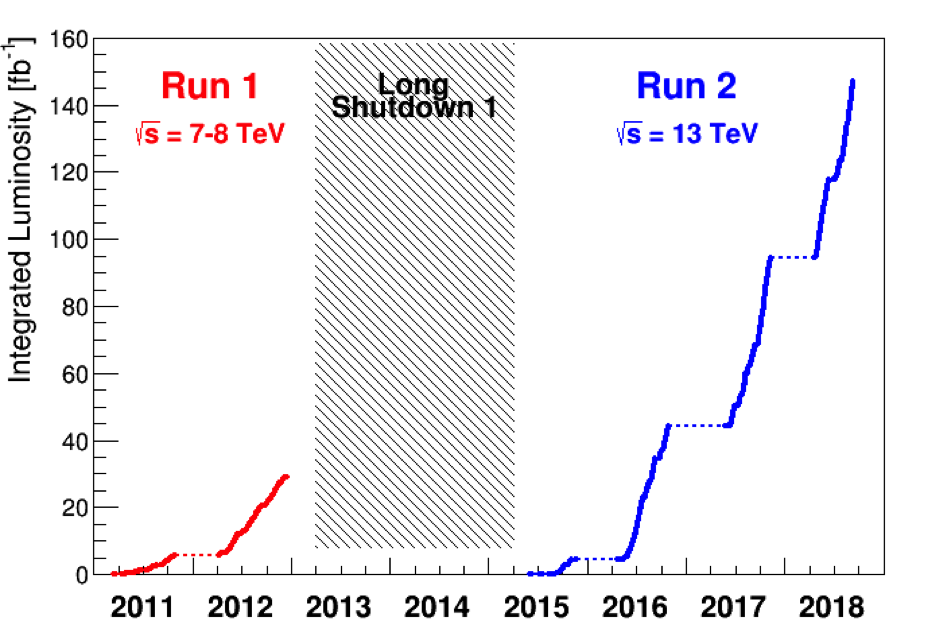
\includegraphics[width=0.5\textwidth]{figure/lhc_lumin.png}
    \caption{Integrated luminosities of Run 1 and Run 2.}
    \label{fig:lhc_lumi}
\end{figure}

\begin{figure}\centering
    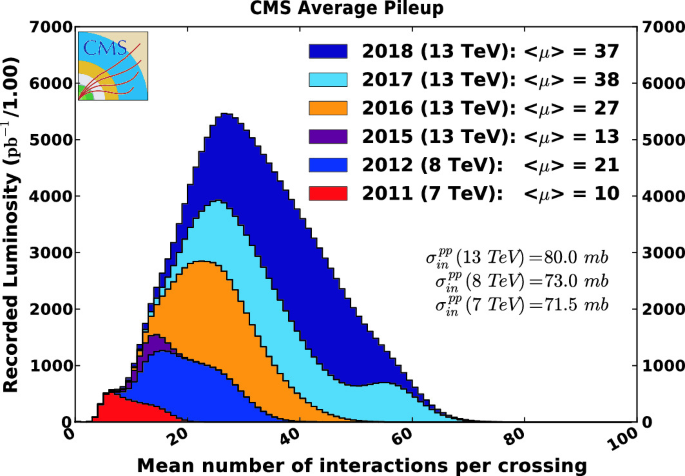
\includegraphics[width=0.5\textwidth]{figure/lhc_pu.png}
    \caption[Average pileup profile for each year of data-taking of the CMS experiment.]
    {Average pileup profile represented in stacked histograms for each year of data-taking of the CMS experiment during the LHC Run 1 and Run 2.}
    \label{fig:lhc_pu}
\end{figure}
